\chapter{Persamaan Schrödinger dan Fungsi Gelombang}\label{ch:b2:schrodinger-wave-functions}

Tembakkanlah elektron satu demi satu ke sepasang celah lalu rekamlah tempat jatuh
masing-masingnya: sebuah titik di sini, sebuah titik di sana, tampaknya acak --- dan sesudah sepuluh
ribu titik, muncullah rumbai percobaan Young, seakan-akan tiap elektronnya
telah melewati kedua celahnya lalu berinterferensi dengan dirinya sendiri. Bab
terakhir jilid Tahun 1 menjumpai keanehan ini: cahaya datang dalam
foton, materi mempunyai panjang gelombang $\lambda = h/p$, dan kedudukan dan
momentumnya tak dapat keduanya tajam. Yang tak diberikannya adalah
\emph{persamaan}-nya --- yaitu kaidah yang mengatakan bagaimana gelombang yang berkaitan dengan sebuah
partikel berkembang, sebagaimana hukum Newton mengatakan bagaimana sebuah lintasan berkembang. Persamaan
itu adalah persamaan Schrödinger (1926), dan dengannya lukisan kuantumnya
menjadi sebuah teori yang dapat dihitung: orang menuliskan sebuah \emph{\omterm{def:b2:schrodinger-wave-functions:psi}{fungsi gelombang}}
$\psi(x,t)$, yang kuadrat modulusnya adalah peluang menemukan
partikelnya, lalu menyelesaikan sebuah persamaan diferensial parsial yang linear. Bab
ini menyatakan persamaannya, menjelaskan apa arti $\psi$ dan apa yang bukan
artinya, mencari \omterm{thm:b2:schrodinger-wave-functions:stationary}{keadaan tegar} dan \omterm{prop:b2:dispersion-wave-packets:group}{paket gelombang} partikel bebasnya,
lalu menunjukkan di mana mekanika Newton muncul kembali --- bagi
segala yang lebih berat daripada sebuah molekul.

\begin{omfigure}
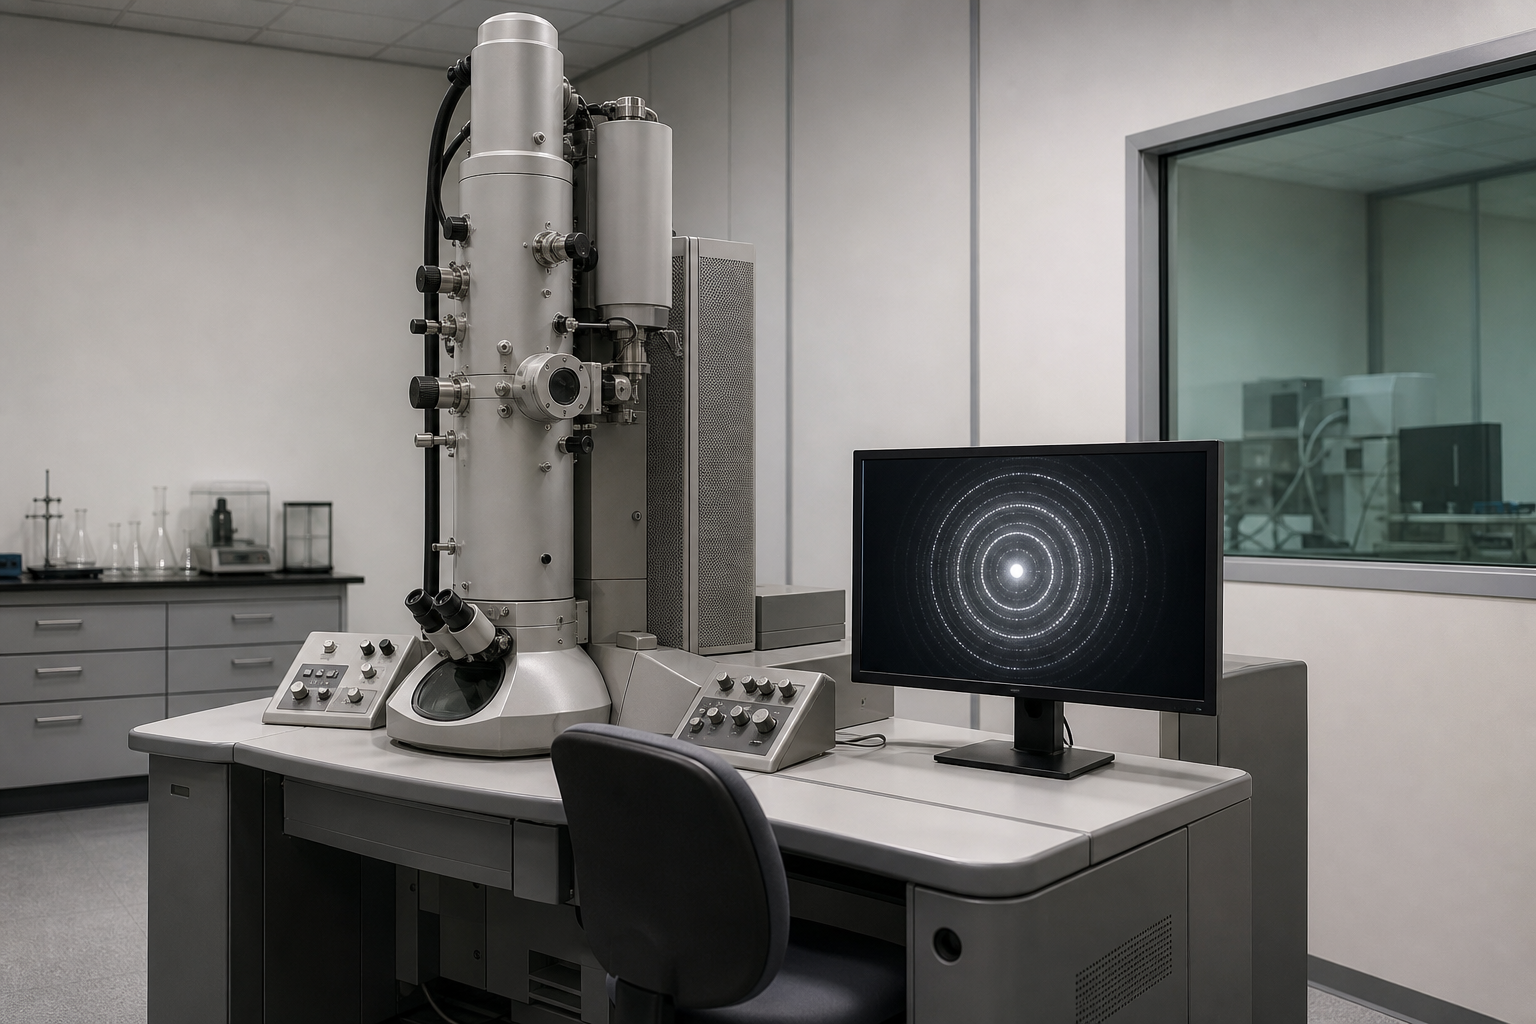
\includegraphics[width=0.58\linewidth]{images/book4/ai/b4-30-electron-microscope.png}

{\small Sebuah mikroskop elektron transmisi: elektron yang dipercepat sampai
seratus kilovolt mempunyai panjang gelombang beberapa pikometer, dan
\omterm{def:b2:schrodinger-wave-functions:psi}{fungsi gelombangnya}, yang difokuskan lensa magnet, mencitrakan atom sebuah
hablur.}
\end{omfigure}

\section{Apa yang ditinggalkan jilid Tahun 1 bagi kita}

\begin{proposition}[Partikel adalah gelombang]\label{prop:b2:schrodinger-wave-functions:recap}
Sebuah foton berfrekuensi $\nu$ mempunyai energi $E = h\nu = \hbar\omega$ dan
momentum $p = h/\lambda = \hbar k$; sebuah partikel bermateri bermomentum $p$
berperilaku sebagai sebuah gelombang berpanjang gelombang $\lambda = h/p$ (de Broglie), dengan $E =
\hbar\omega$ dan $p = \hbar k$ juga --- \omterm{def:b2:diffraction:huygens}{difraksi} elektron oleh
hablur, interferometri neutron dan bahkan molekul mengukuhkannya; dan tak ada
keadaan yang dapat mempunyai kedudukan dan momentum yang lebih tajam daripada $\Delta x\,\Delta p
\ge \hbar/2$ (Heisenberg). Dengan $\hbar = h/2\pi = \qty{1.05e-34}{J.s}$: sebuah
elektron pada \qty{100}{eV} mempunyai $\lambda = \qty{0.12}{nm}$, seukuran sebuah
atom; sebutir debu \qty{1e-15}{kg} pada \qty{1}{mm/s} mempunyai $\lambda =
\qty{7e-16}{m}$, lebih kecil daripada sebuah inti --- ia berperilaku klasik.
\end{proposition}

\begin{proof}
Diingat kembali dari jilid Tahun 1; tugasnya kini adalah dinamika
gelombangnya.
\end{proof}

\begin{omfigure}
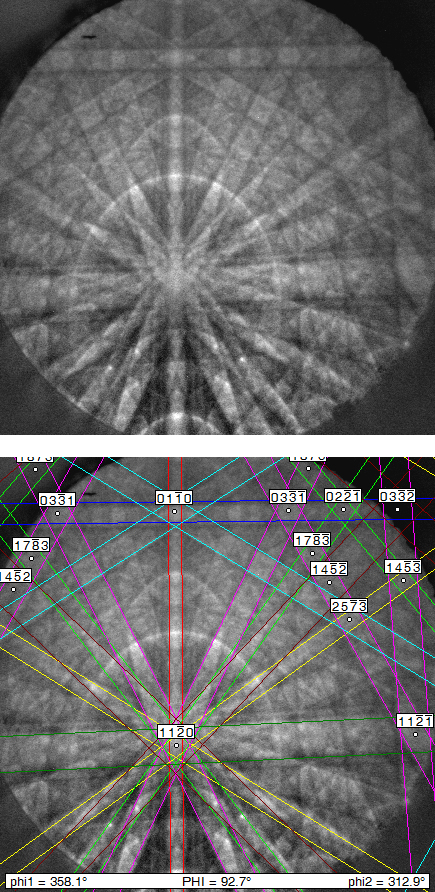
\includegraphics[width=0.4\linewidth, viewport=0 214 209 428, clip]{images/book4/electron-diffraction-nist.jpg}

{\small Sebuah pola \omterm{def:b2:diffraction:huygens}{difraksi} elektron yang direkam dalam sebuah mikroskop elektron (sebuah pola Kikuchi dari sebuah hablur): elektron berpanjang gelombang beberapa pikometer, yang didifraksikan bidang atomnya --- materi yang berperilaku sebagai gelombang (NIST).}
\end{omfigure}

\section{Fungsi gelombang}

\begin{definition}[Fungsi gelombang dan kaidah Born]\label{def:b2:schrodinger-wave-functions:psi}
Keadaan sebuah partikel yang bergerak sepanjang $x$ dilukiskan sebuah
\emph{fungsi gelombang}\index{fungsi gelombang} kompleks $\psi(x,t)$ sedemikian sehingga
\[
\dd\mathcal P = |\psi(x,t)|^2\,\dd x
\]
adalah peluang menemukan partikelnya antara $x$ dan $x + \dd x$
pada saat $t$ (yaitu \emph{kaidah Born}\index{kaidah Born}); maka
\emph{penormalannya} $\int_{-\infty}^{\infty}|\psi|^2\dd x = 1$, dan
nilai harapnya $\langle x\rangle = \int x|\psi|^2\dd x$, $\Delta x^2 =
\langle x^2\rangle - \langle x\rangle^2$. Fungsi gelombang menuruti
\emph{asas tumpang tindih}\index{asas tumpang tindih}: jika
$\psi_1$ dan $\psi_2$ merupakan keadaan yang mungkin, begitu pula $\alpha\psi_1 +
\beta\psi_2$ (yang dinormalkan), dan peluangnya lalu memuat
suku interferensi $2\operatorname{Re}(\alpha^*\beta\,\psi_1^*\psi_2)$. Sebuah
faktor fase menyeluruh $\eu^{\iu\theta}$ tak mengubah apa pun; sebuah fase nisbi
antara dua komponen yang ditumpangkan mengubah interferensinya.
\end{definition}

\begin{remark}[Apa yang bukan $\psi$]\label{rem:b2:schrodinger-wave-functions:not}
$\psi$ bukan sebuah medan klasik yang tersebar dalam ruang seperti $\vect E$, bukan pula
sebuah awan materi: elektronnya selalu ditemukan utuh, di satu titik.
$\psi$ adalah sebuah \emph{amplitudo peluang}, yaitu objek yang
berinterferensi; hanya $|\psi|^2$ yang teramati, dan hanya secara statistik, lewat
mengulangi percobaannya pada partikel yang disiapkan serupa. Titik
celah gandanya adalah elektron tunggal; rumbainya adalah $|\psi_1 +
\psi_2|^2$.
\end{remark}

\section{Persamaan Schrödinger}

\begin{theorem}[Persamaan Schrödinger]\label{thm:b2:schrodinger-wave-functions:equation}
Sebuah partikel bermassa $m$ dalam energi potensial $V(x)$ mempunyai sebuah \omterm{def:b2:schrodinger-wave-functions:psi}{fungsi
gelombang} yang menuruti
\[
\iu\hbar\,\frac{\partial\psi}{\partial t} = -\frac{\hbar^2}{2m}\,\frac{\partial^2\psi}{\partial x^2} + V(x)\,\psi .
\]
Ia linear (tumpang tindih), berorde pertama dalam waktu (\omterm{def:b2:schrodinger-wave-functions:psi}{fungsi gelombangnya}
pada satu saat menetapkannya pada semua waktu kemudian), dan kompleks ($\psi$
tak dapat nyata: $\iu$-nya hakiki). Ia sebuah \emph{postulat},
yang dibenarkan oleh akibatnya.
\end{theorem}

\begin{proof}
Sebuah motivasi alih-alih sebuah bukti. Sebuah partikel bebas bermomentum tajam
$p = \hbar k$ dan berenergi $E = \hbar\omega$ seharusnya berupa sebuah gelombang bidang $\psi =
A\eu^{\iu(kx - \omega t)}$, yang baginya $\iu\hbar\partial_t\psi = \hbar\omega\psi =
E\psi$ dan $-(\hbar^2/2m)\partial_x^2\psi = (\hbar^2k^2/2m)\psi = (p^2/2m)\psi$.
Hubungan klasiknya $E = p^2/2m$ dengan demikian dihasilkan ulang persamaan
$\iu\hbar\partial_t\psi = -(\hbar^2/2m)\partial_x^2\psi$, dan perumuman alaminya
bagi $E = p^2/2m + V$ menambahkan $V\psi$. Perhatikanlah bahwa
persamaannya harus linear agar berlaku bagi tumpang tindih gelombang bidangnya, dan
berorde pertama dalam waktu dengan sebuah $\iu$ agar $\eu^{-\iu\omega t}$ dan bukan
$\cos\omega t$ yang menjadi kebergantungan waktunya --- sebuah \omterm{thm:b2:waves-on-strings:equation}{persamaan gelombang} yang nyata akan
memberi $E^2 \propto p^4$.
\end{proof}

\begin{proposition}[Kekekalan peluang]\label{prop:b2:schrodinger-wave-functions:current}
Rapat peluangnya $\rho = |\psi|^2$ dan \emph{arus
peluang}\index{arus peluang}
\[
j = \frac{\hbar}{m}\operatorname{Im}\Big(\psi^*\frac{\partial\psi}{\partial x}\Big)
= \frac{\hbar}{2\iu m}\Big(\psi^*\partial_x\psi - \psi\,\partial_x\psi^*\Big)
\]
menuruti $\partial_t\rho + \partial_xj = 0$: peluangnya tak diciptakan maupun
dimusnahkan, dan $\int|\psi|^2\dd x$ tetap sama dengan $1$. Bagi sebuah gelombang bidang
$A\eu^{\iu kx}$, $j = |A|^2\hbar k/m = \rho v$: kerapatan dikalikan kecepatan, seperti bagi
sebarang aliran.
\end{proposition}

\begin{proof}
$\partial_t(\psi^*\psi) = \psi^*\partial_t\psi + \psi\,\partial_t\psi^*$; dari
persamaannya dan konjugatnya, $\partial_t\psi = (\iu\hbar/2m)\partial_x^2\psi -
(\iu/\hbar)V\psi$, $\partial_t\psi^* = -(\iu\hbar/2m)\partial_x^2\psi^* +
(\iu/\hbar)V\psi^*$; suku $V$-nya saling meniadakan dan sisanya adalah $(\iu\hbar/2m)(\psi^*
\partial_x^2\psi - \psi\,\partial_x^2\psi^*) = -\partial_xj$.
\end{proof}

\begin{proposition}[Momentum, nilai harap dan limit klasiknya]\label{prop:b2:schrodinger-wave-functions:ehrenfest}
Momentum sebuah keadaan diperoleh lewat operator $\hat p =
-\iu\hbar\,\partial_x$ (yang memberi $\hbar k$ pada sebuah gelombang bidang): $\langle
p\rangle = \int\psi^*(-\iu\hbar\partial_x\psi)\dd x$, dan energinya lewat $\hat H
= -(\hbar^2/2m)\partial_x^2 + V$. Nilai harapnya menuruti
(Ehrenfest)
\[
\frac{\dd\langle x\rangle}{\dd t} = \frac{\langle p\rangle}{m}, \qquad
\frac{\dd\langle p\rangle}{\dd t} = -\Big\langle\frac{\dd V}{\dd x}\Big\rangle :
\]
pusat \omterm{prop:b2:dispersion-wave-packets:group}{paket gelombangnya} menuruti hukum Newton secara eksak ketika $V$
paling banter kuadratik, dan secara hampiran kapan pun paketnya sempit
dibandingkan dengan skala yang sepanjangnya $V$ berubah --- yaitu limit klasiknya,
yang berlaku bagi sebarang objek makroskopis karena $\hbar$ begitu kecil.
\end{proposition}

\begin{proof}
Turunkanlah $\langle x\rangle = \int x|\psi|^2$, pakailah $\partial_t\rho =
-\partial_xj$ lalu integralkanlah bagian demi bagian: $\dd\langle x\rangle/\dd t = \int j\,\dd x
= \langle p\rangle/m$. Hubungan keduanya adalah perhitungan yang sama satu
orde lebih tinggi (diterima tanpa bukti di sini).
\end{proof}

\section{Keadaan tegar}

\begin{theorem}[Keadaan tegar]\label{thm:b2:schrodinger-wave-functions:stationary}
Jika $V$ tak bergantung waktu, persamaannya mempunyai penyelesaian berbentuk
terpisah
\[
\psi(x,t) = \varphi(x)\,\eu^{-\iu Et/\hbar}, \qquad
-\frac{\hbar^2}{2m}\,\varphi'' + V\varphi = E\varphi
\]
(yaitu \emph{persamaan Schrödinger tak bergantung waktu}\index{persamaan
Schrödinger!tak bergantung waktu}): yaitu \emph{keadaan tegar}\index{keadaan
tegar}, yang berenergi $E$ terdefinisi baik, yang rapat peluangnya
$|\varphi|^2$ tak beranjak. Energi $E$ yang $\varphi$-nya
dapat diterima (terbatas, dapat dinormalkan bagi sebuah keadaan terikat) adalah
\emph{aras energi}-nya; penyelesaian umumnya adalah sebuah tumpang tindih $\psi =
\sum_nc_n\varphi_n(x)\eu^{-\iu E_nt/\hbar}$, dan sebuah tumpang tindih dua aras
mempunyai kerapatan yang berayun pada \emph{frekuensi Bohr}\index{frekuensi
Bohr} $\nu_{21} = (E_2 - E_1)/h$ --- yaitu frekuensi cahaya yang
dipancarkan atau diserap atomnya.
\end{theorem}

\begin{proof}
Sisipkanlah $\varphi(x)f(t)$: $\iu\hbar f'/f = (-\hbar^2\varphi''/2m + V\varphi)/\varphi$,
sebuah fungsi $t$ yang sama dengan sebuah fungsi $x$, maka sebuah tetapan $E$; $f
= \eu^{-\iu Et/\hbar}$. Bagi dua aras, $|c_1\varphi_1\eu^{-\iu E_1t/\hbar} +
c_2\varphi_2\eu^{-\iu E_2t/\hbar}|^2 = |c_1\varphi_1|^2 + |c_2\varphi_2|^2 +
2\operatorname{Re}(c_1^*c_2\varphi_1^*\varphi_2\eu^{-\iu(E_2 - E_1)t/\hbar})$.
Kelengkapan \omterm{thm:b2:schrodinger-wave-functions:stationary}{keadaan tegarnya} diterima tanpa bukti.
\end{proof}

\begin{omfigure}
\begin{tikzpicture}
  \begin{axis}[omaxis, width=7.4cm, height=4.4cm, xmin=0, xmax=1, ymin=-1.3, ymax=1.5,
    xlabel={$x/L$}, ylabel={$\psi$}, xtick={0.5,1}, ytick=\empty, clip=false,
    legend style={font=\scriptsize, at={(0.5,-0.28)}, anchor=north, draw=none, fill=none, legend columns=3}]
    \addplot[omDef, thick, domain=0:1, samples=80] {1.41*sin(deg(pi*x))*cos(40)};
    \addlegendentry{$\operatorname{Re}\psi$}
    \addplot[omExo, thick, dashed, domain=0:1, samples=80] {-1.41*sin(deg(pi*x))*sin(40)};
    \addlegendentry{$\operatorname{Im}\psi$}
    \addplot[omThm, thick, domain=0:1, samples=80] {2*sin(deg(pi*x))^2-1.3};
    \addlegendentry{$|\psi|^2$ (tergeser)}
  \end{axis}
  \begin{scope}[xshift=9.4cm, yshift=1.3cm, >=stealth]
    \draw[->] (-1.5,0) -- (1.5,0) node[right, font=\scriptsize] {Re};
    \draw[->] (0,-1.5) -- (0,1.5) node[above, font=\scriptsize] {Im};
    \draw[gray] (0,0) circle (1.1);
    \draw[->, omDef, very thick] (0,0) -- (-40:1.1);
    \draw[->, omDef] (1.1,0) arc (0:-40:1.1);
    \node[font=\scriptsize, omDef] at (-50:1.55) {$-Et/\hbar$};
    \node[font=\scriptsize] at (0,-1.85) {$\eu^{-\iu Et/\hbar}$};
  \end{scope}
\end{tikzpicture}

{\small Sebuah \omterm{thm:b2:schrodinger-wave-functions:stationary}{keadaan tegar}: profil ruangnya $\varphi(x)$ (di sini
keadaan dasar sebuah sumur) dikalikan sebuah fasor yang berputar dengan laju
$E/\hbar$; bagian nyata dan khayalnya berputar saling masuk sementara
$|\psi|^2$ tetap diam.}
\end{omfigure}

\begin{omfigure}
\begin{tikzpicture}
  \begin{axis}[omaxis, width=9cm, height=4.4cm, xmin=0, xmax=1, ymin=0, ymax=2.6,
    xlabel={$x/L$}, ylabel={$|\psi|^2$}, xtick={0.5,1}, ytick=\empty, clip=false,
    legend style={font=\scriptsize, at={(0.5,-0.28)}, anchor=north, draw=none, fill=none, legend columns=3}]
    \addplot[omDef, thick, domain=0:1, samples=100] {(sin(deg(pi*x)))^2 + (sin(deg(2*pi*x)))^2 + 2*sin(deg(pi*x))*sin(deg(2*pi*x))};
    \addlegendentry{$t = 0$}
    \addplot[omThm, thick, dashed, domain=0:1, samples=100] {(sin(deg(pi*x)))^2 + (sin(deg(2*pi*x)))^2};
    \addlegendentry{$t = T_{21}/4$}
    \addplot[omExo, thick, domain=0:1, samples=100] {(sin(deg(pi*x)))^2 + (sin(deg(2*pi*x)))^2 - 2*sin(deg(pi*x))*sin(deg(2*pi*x))};
    \addlegendentry{$t = T_{21}/2$}
  \end{axis}
\end{tikzpicture}

{\small Sebuah tumpang tindih kedua keadaan terendah sebuah sumur:
kerapatannya berkecipak dari satu sisi ke sisi lainnya pada \omterm{thm:b2:schrodinger-wave-functions:stationary}{frekuensi Bohr}
$(E_2 - E_1)/h$ --- sebuah muatan yang berayun, maka (\cref{ch:b2:dipole-radiation})
sebuah dwikutub yang memancar tepat pada frekuensi garis spektrumnya.}
\end{omfigure}

\section{Partikel bebas: gelombang bidang dan paket gelombang}

\begin{proposition}[Partikel bebas]\label{prop:b2:schrodinger-wave-functions:free}
Bagi $V = 0$ \omterm{thm:b2:schrodinger-wave-functions:stationary}{keadaan tegarnya} adalah gelombang bidang $\eu^{\iu(kx -
\omega t)}$ dengan
\[
E = \hbar\omega = \frac{\hbar^2k^2}{2m}, \qquad
v_\varphi = \frac{\omega}{k} = \frac{\hbar k}{2m}, \qquad
v_{\text{g}} = \frac{\dd\omega}{\dd k} = \frac{\hbar k}{m} = \frac{p}{m} :
\]
gelombang materi bersifat \emph{dispersif}; \omterm{def:b2:dispersion-wave-packets:relation}{kecepatan fasenya} tak mempunyai
makna fisis, dan \emph{\omterm{prop:b2:dispersion-wave-packets:group}{kecepatan grup}}-nya adalah kecepatan partikelnya. Sebuah gelombang
bidang tak dapat dinormalkan --- sebuah partikel bermomentum tajam sempurna
tersebar di seluruh ruang --- sehingga sebuah partikel yang sungguhan adalah sebuah \emph{paket
gelombang}\index{paket gelombang}, yaitu sebuah tumpang tindih gelombang bidang pada sebuah pita
$\Delta k$, yang terlokalkan sepanjang $\Delta x \sim 1/\Delta k$, bergerak dengan $v_{\text{g}}$ dan
\emph{menyebar}: sebuah paket Gauss berlebar awal $\sigma_0$ mempunyai pada
saat $t$ lebar
\[
\sigma(t) = \sigma_0\sqrt{1 + \Big(\frac{\hbar t}{2m\sigma_0^2}\Big)^2}, \qquad
\tau = \frac{2m\sigma_0^2}{\hbar} ,
\]
dan memenuhi $\Delta x\,\Delta p = \hbar/2$ pada $t = 0$ (yaitu minimum yang dibolehkan)
dan lebih daripadanya kemudian.
\end{proposition}

\begin{proof}
\omterm{def:b2:dispersion-wave-packets:relation}{Hubungan dispersinya} menyusul dari persamaannya; $v_{\text{g}}$ seperti dalam
\cref{ch:b2:dispersion-wave-packets}. Rumus penyebarannya datang dari
sintesis Fourier paketnya --- tiap komponen $\eu^{\iu kx}$ memungut
fase $\eu^{-\iu\hbar k^2t/2m}$, dan integral Gauss dengan sebuah
koefisien kompleks memberi sebuah Gauss berlebar tumbuh; integral
Fouriernya adalah perkakas jilid matematika Tahun 3 dan kita menerima
hasilnya. Secara fisis: paketnya memuat momentum yang tersebar pada $\Delta p
= \hbar/2\sigma_0$, maka kecepatan yang tersebar pada $\Delta v = \hbar/2m\sigma_0$,
dan sesudah $t$ komponen yang lebih cepat telah melampaui yang lebih lambat sebesar $\Delta v\,t$
--- rumusnya mengatakan tepat inilah.
\end{proof}

\begin{omfigure}
\begin{tikzpicture}
  \begin{axis}[omaxis, width=6.2cm, height=4.4cm, xmin=0, xmax=3, ymin=0, ymax=2.6,
    xlabel={$k$}, ylabel={$\omega$}, xtick=\empty, ytick=\empty, clip=false]
    \addplot[omDef, thick, domain=0:2.3, samples=60] {x*x/2};
    \addplot[omExo, dashed, domain=0.4:2.6] {1.5*x-1.125};
    \addplot[omThm, dashed, domain=0:2.8] {0.75*x};
    \fill (axis cs:1.5,1.125) circle (1.5pt);
    \node[font=\scriptsize, omExo, anchor=west] at (axis cs:0.15,2.5) {$v_{\text{g}} = \hbar k/m$ (garis singgung)};
    \node[font=\scriptsize, omThm, anchor=west] at (axis cs:2.3,1.5) {$v_\varphi = \hbar k/2m$};
    \node[font=\scriptsize] at (axis cs:0.8,1.5) {$\omega = \hbar k^2/2m$};
  \end{axis}
  \begin{axis}[omaxis, width=7cm, height=4.4cm, xmin=-2.5, xmax=10, ymin=0, ymax=1.15, xshift=6.8cm,
    xlabel={$x/\sigma_0$}, ylabel={$|\psi|^2$}, xtick=\empty, ytick=\empty, clip=false]
    \addplot[omDef, thick, domain=-2.5:10, samples=120] {exp(-(x-1)^2/2)};
    \addplot[omThm, thick, domain=-2.5:10, samples=120] {(1/1.41)*exp(-(x-3.5)^2/4)};
    \addplot[omExo, thick, domain=-2.5:10, samples=120] {(1/2.24)*exp(-(x-6)^2/10)};
    \node[font=\scriptsize, omDef, anchor=west] at (axis cs:1.3,1.0) {$t = 0$};
    \node[font=\scriptsize, omThm, anchor=west] at (axis cs:3.8,0.75) {$\tau$};
    \node[font=\scriptsize, omExo, anchor=west] at (axis cs:6.3,0.5) {$2\tau$};
  \end{axis}
\end{tikzpicture}

{\small Kiri: kurva dispersi partikel bebasnya, dengan \omterm{prop:b2:dispersion-wave-packets:group}{kecepatan
grupnya} (garis singgung) dan \omterm{def:b2:dispersion-wave-packets:relation}{kecepatan fasenya} (talibusur ke titik asalnya), separuhnya.
Kanan: sebuah paket Gauss yang bergerak dengan $v_{\text{g}}$ lalu menyebar
--- lebarnya $\sqrt2$ kali lebih besar sesudah $\tau = 2m\sigma_0^2/\hbar$, puncaknya
lebih rendah, luasnya tetap.}
\end{omfigure}

\begin{example}[Siapa yang menyebar]\label{ex:b2:schrodinger-wave-functions:spreading}
Sebuah elektron yang terlokalkan dalam $\sigma_0 = \qty{1}{nm}$: $\tau = 2m\sigma_0^2/\hbar
= \qty{1.7e-14}{s}$ --- sesudah senanosekon paketnya selebar \qty{60}{\micro m}:
sebuah elektron yang ditinggal sendirian tak tinggal diam; yang terikat dalam sebuah atom ia
tak menyebar karena potensialnya menahannya (yaitu sebuah \omterm{thm:b2:schrodinger-wave-functions:stationary}{keadaan tegar}).
Sebutir debu \qty{1e-15}{kg} yang terlokalkan sampai \qty{1}{\micro m}: $\tau =
\qty{2e7}{s}$, delapan bulan; sebutir peluru: lebih lama daripada umur alam semesta.
Penyebaran kuantumnya nyata, dan tak tampak bagi apa pun yang dapat dilihat orang.
\end{example}

\begin{remark}[Energi dan waktu]\label{rem:b2:schrodinger-wave-functions:energytime}
Sebuah keadaan yang hanya ada selama $\Delta t$ --- sebuah atom tereksitasi berumur
$\tau$, sebuah \omterm{prop:b2:scalar-light-model:coherence}{deret gelombang} sepanjang $c\tau$ --- adalah sebuah tumpang tindih energi
yang tersebar pada $\Delta E \sim \hbar/\Delta t$: yaitu hubungan Fourier
\cref{ch:b2:scalar-light-model} antara durasi sebuah deret dan
\omterm{prop:b2:scalar-light-model:coherence}{lebar spektrumnya}, yang kini diterapkan pada $E = \hbar\omega$. Sebuah aras atomik berumur
\qty{10}{ns} mempunyai lebar $\Delta E = \qty{7e-8}{eV}$, yaitu sebuah
lebar garis alami \qty{16}{MHz}; lebar Doppler \cref{ch:b2:laser}
(\qty{1.5}{GHz}) menyembunyikannya dalam sebuah gas, tetapi tidak dalam sebuah atom dingin atau sebuah ion yang
diam.
\end{remark}

\begin{method}[Bekerja dengan fungsi gelombang]\label{meth:b2:schrodinger-wave-functions:method}
(1) Normalkanlah; peluangnya adalah $\int|\psi|^2$ pada daerahnya. (2)
$V$ yang tak bergantung waktu: carilah $\varphi(x)\eu^{-\iu Et/\hbar}$, selesaikanlah
persamaan tegarnya, paksakanlah syarat batasnya --- itulah arasnya.
(3) Tumpangkanlah \omterm{thm:b2:schrodinger-wave-functions:stationary}{keadaan tegarnya} bagi perkembangannya; dua arasnya berlayang pada
$(E_2 - E_1)/h$. (4) Gerak bebas: $v_{\text{g}} = p/m$, waktu penyebarannya
$2m\sigma_0^2/\hbar$. (5) Arus: $j = (\hbar/m)\operatorname{Im}(\psi^*\psi')$;
bagi $A\eu^{\iu kx} + B\eu^{-\iu kx}$, $j = (|A|^2 - |B|^2)\hbar k/m$ (tanpa suku silang).
(6) Limit klasik: Ehrenfest, dan $\lambda$ terhadap ukuran
radasnya.
\end{method}

\section{Latihan}

\begin{exercise}[$\star$]\label{exo:b2:schrodinger-wave-functions:1}
Tentukanlah panjang gelombang de Broglie: sebuah elektron pada \qty{100}{eV}, \qty{10}{keV},
\qty{100}{keV} (pakailah $p = \sqrt{2mE}$, lalu katakanlah mengapa yang terakhir menuntut sebuah
koreksi); sebuah neutron termal (\qty{25}{meV}, $m = \qty{1.67e-27}{kg}$); sebuah
molekul C$_{60}$ ($m = \qty{1.2e-24}{kg}$) pada \qty{200}{m/s}; sebuah bola
tenis. Mana di antaranya yang menunjukkan interferensi?
\end{exercise}

\begin{exercise}[$\star$]\label{exo:b2:schrodinger-wave-functions:2}
$\psi(x) = A\eu^{-x^2/2a^2}$: tentukanlah $A$ (pakailah $\int\eu^{-u^2}\dd u = \sqrt\pi$);
$\langle x\rangle$, $\Delta x$; peluang menemukan partikelnya dalam
$|x| < a$ ($\operatorname{erf}(1) = 0.84$) dan dalam $|x| < 2a$ ($0.9995$).
\end{exercise}

\begin{exercise}[$\star$]\label{exo:b2:schrodinger-wave-functions:3}
Periksalah bahwa $\varphi(x)\eu^{-\iu Et/\hbar}$ menyelesaikan persamaannya ketika $\varphi$
menyelesaikan yang tegar. Tentukanlah frekuensi fasornya bagi $E = \qty{1}{eV}$;
bagi sebuah tumpang tindih dua aras yang terpisah \qty{2}{eV}, frekuensi dan
panjang gelombang ayunan $|\psi|^2$-nya --- dan panjang gelombang cahaya yang
dipancarkan.
\end{exercise}

\begin{exercise}[$\star$]\label{exo:b2:schrodinger-wave-functions:4}
Tentukanlah waktu penyebaran $\tau = 2m\sigma_0^2/\hbar$ dan lebarnya sesudah \qty{1}{ns} dan
\qty{1}{s}: bagi sebuah elektron ber-$\sigma_0 = \qty{1}{nm}$ dan $\sigma_0 = \qty{1}{mm}$;
bagi sebuah proton ber-$\sigma_0 = \qty{1}{nm}$; bagi sebutir \qty{1e-12}{kg} dengan
$\sigma_0 = \qty{1}{\micro m}$. Mengapa benda tetap di tempat ia ditaruh?
\end{exercise}

\begin{exercise}[$\star\star$]\label{exo:b2:schrodinger-wave-functions:5}
\emph{Arus.} (a) Turunkanlah persamaan kontinuitasnya. (b) Tentukanlah $j$ bagi
$A\eu^{\iu kx}$, bagi $A\sin kx$, bagi $A\eu^{\iu kx} + B\eu^{-\iu kx}$. (c) Mengapa
ketiadaan sebuah suku silang pada hal yang terakhir merupakan pernyataan bahwa
fluks pantul dan datangnya sekadar berkurangan? (d) Tunjukkanlah bahwa bagi sebuah \omterm{def:b2:schrodinger-wave-functions:psi}{fungsi
gelombang} yang nyata $j = 0$: sebuah \omterm{thm:b2:schrodinger-wave-functions:stationary}{keadaan tegar} yang terikat tak mengemban arus.
\end{exercise}

\begin{exercise}[$\star\star$]\label{exo:b2:schrodinger-wave-functions:6}
\emph{Sebuah paket Gauss.} $\psi(x,0) = A\eu^{\iu k_0x}\eu^{-x^2/4\sigma^2}$. (a)
Tentukanlah $A$, $\langle x\rangle$, $\Delta x$. (b) $\langle p\rangle$ dengan $\hat p =
-\iu\hbar\partial_x$. (c) Dengan menerima $\Delta p = \hbar/2\sigma$, periksalah
$\Delta x\Delta p = \hbar/2$. (d) Buktikanlah $\dd\langle x\rangle/\dd t = \langle
p\rangle/m$ dari persamaan kontinuitasnya.
\end{exercise}

\begin{exercise}[$\star\star$]\label{exo:b2:schrodinger-wave-functions:7}
\emph{Elektron dalam sebuah tabung.} Elektron yang dipercepat menembus \qty{100}{V}
menyeberangi \qty{30}{cm}. (a) Tentukanlah kelajuannya, panjang gelombangnya, waktu terbangnya. (b) \omterm{def:b2:dispersion-wave-packets:relation}{Kecepatan fase} dan
grupnya; yang mana kecepatan elektronnya? (c) Sebuah paket yang mula-mula
selebar \qty{10}{\micro m}: berapa waktu penyebarannya, lebarnya saat tiba. (d) \omterm{def:b2:diffraction:huygens}{Difraksi}
oleh sebuah apertur \qty{0.3}{mm} di jalannya: berapa sebaran sudut dan bintiknya pada
layarnya. Sahihkah gambaran sinarnya?
\end{exercise}

\begin{exercise}[$\star\star$]\label{exo:b2:schrodinger-wave-functions:8}
\emph{Fase.} (a) Tunjukkanlah bahwa $\psi$ dan $\eu^{\iu\theta}\psi$ memberi ramalan
yang sama. (b) Bagi $\psi = (\psi_1 + \eu^{\iu\alpha}\psi_2)/\sqrt2$, tuliskanlah
$|\psi|^2$ lalu tunjukkanlah bahwa $\alpha$ berarti. (c) Dalam celah gandanya, apa
itu $\psi_1$ dan $\psi_2$, dan apa yang menetapkan fase nisbinya di sebuah titik
layarnya? (d) Mengapa mendeteksi celah mana yang dilewati elektronnya
merusak rumbainya (secara kualitatif)?
\end{exercise}

\begin{exercise}[$\star\star$]\label{exo:b2:schrodinger-wave-functions:9}
\emph{Ehrenfest.} (a) Bagi $V = \tfrac12m\omega^2x^2$, tunjukkanlah bahwa $\langle
x\rangle$ menuruti secara eksak $\ddot{\langle x\rangle} = -\omega^2\langle x\rangle$.
(b) Bagi $V = mgx$, $\langle x\rangle$ jatuh seperti sebuah batu. (c) Bagi sebuah
$V$ yang umum, kapan $\langle V'(x)\rangle \approx V'(\langle x\rangle)$? (d) Sebuah
manik \qty{1}{g} dalam sebuah mangkuk: taksirlah ukuran paketnya yang diperlukan agar
ia menjadi ``kuantum'' lalu bandingkanlah dengan sebuah atom.
\end{exercise}

\begin{exercise}[$\star\star\star$]\label{exo:b2:schrodinger-wave-functions:10}
\emph{Berkecipak.} Dalam sebuah kotak $0 < x < L$ berdinding yang tak tertembus
\omterm{thm:b2:schrodinger-wave-functions:stationary}{keadaan tegarnya} adalah $\varphi_n = \sqrt{2/L}\sin(n\pi x/L)$, $E_n =
n^2h^2/8mL^2$ (\cref{ch:b2:potential-wells-tunneling}). Ambillah $\psi =
(\varphi_1\eu^{-\iu E_1t/\hbar} + \varphi_2\eu^{-\iu E_2t/\hbar})/\sqrt2$. (a)
Tentukanlah $|\psi|^2$ sebagai fungsi waktu. (b) Tunjukkanlah $\langle x\rangle = L/2 -
(16L/9\pi^2)\cos\omega_{21}t$ (pakailah $\int_0^L x\sin(\pi x/L)\sin(2\pi x/L)\dd x
= -8L^2/9\pi^2$). (c) Elektron, $L = \qty{1}{nm}$: tentukanlah $E_2 - E_1$,
frekuensi dan panjang gelombang ayunannya. (d) Apa yang dilakukan sebuah
muatan yang berayun (\cref{ch:b2:dipole-radiation})? Simpulkanlah tentang
garis spektrumnya.
\end{exercise}

\begin{exercise}[$\star\star\star$]\label{exo:b2:schrodinger-wave-functions:11}
\emph{Penyebaran, yang diturunkan.} Paket $\psi(x,0) \propto \eu^{-x^2/4\sigma_0^2}$
adalah tumpang tindih $\int g(k)\eu^{\iu kx}\dd k$ dengan $g(k) \propto
\eu^{-\sigma_0^2k^2}$ (diterima tanpa bukti: transformasi Fourier sebuah Gauss adalah sebuah
Gauss, berlebar $1/2\sigma_0$ dalam $k$). (a) Tuliskanlah $\psi(x,t)$ dengan memberi tiap
komponennya fasenya $\eu^{-\iu\hbar k^2t/2m}$. (b) Lengkapkanlah kuadratnya dalam
eksponennya lalu terimalah $\int\eu^{-\alpha k^2 + \beta k}\dd k = \sqrt{\pi/\alpha}\,
\eu^{\beta^2/4\alpha}$ bagi $\alpha$ kompleks yang bagian nyatanya positif: tunjukkanlah bahwa
$|\psi|^2$ adalah sebuah Gauss berlebar $\sigma(t) = \sigma_0\sqrt{1 + (\hbar t/2m
\sigma_0^2)^2}$. (c) Tafsirkanlah $\tau$ lewat $\Delta v = \Delta p/m$. (d) Mengapa
sebuah paket foton dalam hampa tak menyebar?
\end{exercise}

\begin{exercise}[$\star\star\star$]\label{exo:b2:schrodinger-wave-functions:12}
\emph{Energi--waktu.} (a) Sebuah keadaan yang meluruh sebagai $\eu^{-t/2\tau}\eu^{-\iu E_0t/\hbar}$
(peluangnya $\eu^{-t/\tau}$) adalah sebuah tumpang tindih energi: dengan menerima
bahwa sebaran energinya adalah sebuah Lorentz berlebar penuh $\Gamma =
\hbar/\tau$, berikanlah $\Gamma$ bagi $\tau = \qty{10}{ns}$ (atom), \qty{1e-8}{s},
\qty{1e-23}{s} (sebuah resonansi hadron, dalam MeV). (b) Tentukanlah lebar garis alami
aras \qty{10}{ns}-nya dalam frekuensi; bandingkanlah dengan lebar Doppler
\qty{1.5}{GHz}. (c) Bagaimana orang melihat lebar alaminya (atom dingin,
ion terperangkap)? (d) Kaitkanlah dengan \omterm{prop:b2:scalar-light-model:coherence}{panjang koherensi} \omterm{prop:b2:scalar-light-model:coherence}{deret gelombang}
yang dipancarkan.
\end{exercise}

\section{Soal: Elektron dalam sebuah tabung dan penyebaran sebuah paket gelombang}

\begin{problem}[{Soal akhir pekan --- kapan sebuah elektron menjadi partikel,
kapan menjadi gelombang}]\label{pb:b2:schrodinger-wave-functions:1}
Data: $h = \qty{6.63e-34}{J.s}$, $\hbar = \qty{1.05e-34}{J.s}$, $m_{\text{e}} =
\qty{9.11e-31}{kg}$, $e = \qty{1.60e-19}{C}$, $m_{\text{p}} = \qty{1.67e-27}{kg}$.

\textbf{Bagian I --- Tabung sinar katodenya.}
Elektron meninggalkan sebuah katode panas dengan energi yang dapat diabaikan, dipercepat
menembus $U = \qty{20}{kV}$, melewati sebuah apertur \qty{0.3}{mm}, lalu menumbuk sebuah
layar \qty{40}{cm} jauhnya.
\begin{enumerate}
  \item Kelajuan dan momentumnya (tak relativistik); panjang gelombang de Brogliennya.
  \item Energi kinetiknya $4\%$ dari $mc^2$: dapat diterimakah garapan
        tak relativistiknya bagi soal ini?
  \item Waktu terbangnya ke layarnya.
  \item \omterm{def:b2:diffraction:huygens}{Difraksi} oleh aperturnya: berapa sebaran sudutnya $\sim\lambda/a$ dan
        bintik yang dihasilkannya pada layarnya; bandingkanlah dengan sebuah piksel
        (\qty{0.3}{mm}).
  \item Heisenberg di aperturnya: $\Delta p_y \gtrsim \hbar/2a$ memberi
        sebaran yang sama --- periksalah.
  \item Sebuah paket selebar \qty{0.3}{mm} sepanjang berkasnya: berapa waktu penyebarannya
        $2m\sigma_0^2/\hbar$ dan lebarnya di layarnya.
  \item Keping pembelok menerapkan sebuah gaya melintang: menurut Ehrenfest, bagaimana
        $\langle y\rangle$ beranjak? Simpulkanlah bahwa tabungnya adalah sebuah
        piranti klasik.
  \item \omterm{def:b2:dispersion-wave-packets:relation}{Kecepatan fase} gelombang elektronnya; mengapa bukan paradoks bahwa
        ia berbeda dari kelajuan elektronnya?
\end{enumerate}

\textbf{Bagian II --- \omterm{prop:b2:dispersion-wave-packets:group}{Paket gelombang}.}
\begin{enumerate}[resume]
  \item Bagi sebuah paket Gauss berlebar $\sigma_0$: tentukanlah $\Delta p$ dan
        sebaran kecepatannya $\Delta v$.
  \item Waktu penyebaran bagi sebuah elektron ber-$\sigma_0 = \qty{0.1}{nm}$,
        \qty{1}{nm}, \qty{1}{\micro m}; bagi sebuah proton ber-\qty{1}{nm}; bagi sebuah
        virus (\qty{1e-17}{kg}) ber-\qty{10}{nm}.
  \item Sebuah elektron dalam sebuah atom hidrogen terlokalkan sampai \qty{0.1}{nm}
        lalu tak menyebar: mengapa?
  \item Sebuah elektron bebas pada \qty{1}{eV} ber-$\sigma_0 = \qty{1}{nm}$: sejauh apa
        ia menempuh sebelum lebarnya berlipat dua? Bandingkanlah dengan
        panjang gelombangnya.
  \item Dalam sebuah logam, elektron hantarannya adalah gelombang ber-$\lambda \approx
        \qty{0.5}{nm}$ di seluruh hablurnya: dalam arti apa mereka
        ``terdelokalkan''?
  \item Sebuah mikroskop elektron pada \qty{100}{keV} mempunyai $\lambda \approx
        \qty{4}{pm}$, namun hanya mengurai \qty{0.1}{nm}: mengapa (lensa magnetnya
        menerima setengah sudut sekitar \qty{10}{mrad})?
  \item Berikanlah kriteria yang memutuskan apakah sebuah objek harus
        digarap dengan sebuah \omterm{def:b2:schrodinger-wave-functions:psi}{fungsi gelombang} atau dengan Newton.
\end{enumerate}

\textbf{Bagian III --- \omterm{thm:b2:schrodinger-wave-functions:stationary}{Keadaan tegar} dan transisi.}
Sebuah elektron terkurung dalam $0 < x < L = \qty{1}{nm}$; $\varphi_n =
\sqrt{2/L}\sin(n\pi x/L)$, $E_n = n^2h^2/8mL^2$.
\begin{enumerate}[resume]
  \item Tentukanlah $E_1$, $E_2$, $E_3$ dalam elektronvolt; \omterm{thm:b2:schrodinger-wave-functions:stationary}{frekuensi Bohrnya}
        $\nu_{21}$, $\nu_{31}$ dan panjang gelombangnya.
  \item Periksalah bahwa $|\varphi_n\eu^{-\iu E_nt/\hbar}|^2$ tak bergantung waktu;
        di mana elektronnya paling mungkin dalam keadaan dasarnya?
  \item Bagi $\psi = (\varphi_1\eu^{-\iu E_1t/\hbar} + \varphi_2\eu^{-\iu E_2t/\hbar})/
        \sqrt2$: tentukanlah $|\psi|^2$ pada $t = 0$ dan $t = T_{21}/2$; sketsalah.
  \item Tentukanlah $\langle x\rangle(t)$ (mengingat $\int_0^Lx\varphi_1\varphi_2\dd x = -16L/9\pi^2$):
        berapa amplitudo kecipaknya.
  \item \omterm{thm:b2:dipole-radiation:field}{Dwikutub berayun} $e\langle x\rangle$ memancar: pada frekuensi yang
        mana, dan apa yang dikatakannya tentang garis spektrum dan
        tentang kemantapan \omterm{thm:b2:schrodinger-wave-functions:stationary}{keadaan tegarnya}?
  \item Energi keadaan $\psi$-nya: adakah ia $E_1$, $E_2$, atau sesuatu yang
        lain? Apa yang diberikan sebuah pengukuran?
\end{enumerate}

\textbf{Bagian IV --- Tafsirannya.}
\begin{enumerate}[resume]
  \item Dalam percobaan celah ganda elektron tunggalnya, apa yang acak
        dan apa yang tidak?
  \item Tuliskanlah \omterm{prop:b2:schrodinger-wave-functions:current}{arus peluang} $A\eu^{\iu kx}$ lalu kaitkanlah ia dengan
        sebuah berkas $n$ elektron tiap satuan panjang berkelajuan $v$.
  \item Mengapa persamaan Schrödinger harus kompleks dan berorde pertama
        dalam waktu (dua alasan)?
  \item Ringkaslah dalam lima baris: \omterm{def:b2:schrodinger-wave-functions:psi}{fungsi gelombangnya}, persamaannya,
        \omterm{thm:b2:schrodinger-wave-functions:stationary}{keadaan tegarnya}, paketnya, limit klasiknya.
\end{enumerate}
\end{problem}
